\section{Solutions}
\label{sec:Solutions}

This section presents solutions to the Families-to-Per\-sons benchmark submitted to the Transformation Tool Contest 2017 \cite{Anjorin2017a}.
The solutions have been selected to cover a wide spectrum of bx approaches, implemented in different tools and languages.
Some of them (BiGUL, BXtend, and eMoflon) were provided as reference solutions to the TTC 2017 participants. The solutions in EVL+STrace, NMF Synchronizations, and SDMLib were submitted to TTC 2017 and were published in the TTC proceedings \cite{Hinkel2017,Samimi-Dehkordi2017,Zundorf2017}.
The JTL solution was prepared after the TTC. 

A summary of a classification of these seven solutions based on our feature model is provided in table~\ref{tab:features-all-tools}.
In the following subsections, one for each tool/solution in alphabetical order, we shall refer to this table and explain each tool's classification in detail.

\renewcommand{\arraystretch}{1.2}

\newcolumntype{P}[1]{>{\centering\arraybackslash}p{#1}}
\newcolumntype{M}[1]{>{\centering\arraybackslash}m{#1}}
\begin{table*}[!tbp]
\begin{tabular}{M{1.55cm}|M{1.7cm}|M{1.6cm}|M{1.9cm}|M{2.1cm}|M{1.7cm}|M{1.7cm}|M{1.5cm}}
\textit{} & \textbf{BiGUL} & \textbf{BXtend} & \textbf{eMoflon} & \textbf{EVL+STrace} & \textbf{JTL} & \textbf{NMF} & \textbf{SDMLib} \\ \hline
\textit{Style (Tool)} & restoration-based & restoration-based & propagation-based & restoration-based & restoration-based & propagation-based &  restoration-based \\ \hline
\textit{Scenario (Solution)} & initial-state-based (with~hAln) & initial-diag-based & s-delta-corr-based & initial-diag-based & initial-diag-based & o-delta-corr-based &  initial-diag-based \\ \hline
\textit{Guarantees (Tool)} & round-trip laws & none & correctness, completeness & none & correctness, hippocraticness & correctness, hippocraticness &  none \\ \hline
\textit{Consistency (Tool)} & implicit & implicit & explicit (grammar-based) & explicit (constraint-based) & explicit (constraint-based) & explicit (constraint-based) &  implicit \\ \hline 
\textit{Control (Tool)} & explicit and implicit & explicit & implicit & explicit & implicit & explicit and implicit & explicit \\ \hline
\textit{Direction (Tool)} & directed & directed & directed & concurrent & directed & directed & directed \\ \hline
\textit{Time (Solution)} & on-demand & on-demand & on-demand & on-demand & on-demand & live & on-demand \\ \hline
\textit{Automation (Solution)} & automatic & automatic & automatic & interactive & automatic & automatic & automatic \\
\end{tabular}
\caption{Summary of classification of all tools and solutions}
\label{tab:features-all-tools}
\end{table*}

\subsection{BiGUL}
\label{sec:BiGUL}

\NOTE{\emph{Solution expert:} Josh, \emph{Interviewer:} Tony}

% History, website, tutorial, community
BiGUL~\cite{PEPM2016-Ko}, short for \emph{the Bidirectional Generic Update Language}, is the current result of a long line of research on \emph{bidirectional programming}~\cite{Foster2012} predominantly performed by the programming language community.
Bidirectional programming languages typically share two main ideas in common:  (i)~the task of programming a bx can be reduced by automatically deriving one direction of synchronization from the other direction that is explicitly programmed, and (ii)~well-behavedness properties are guaranteed by providing a small set of well-behaved primitive functions, and combinators to allow bx programmers to compose complex, well-behaved bidirectional programs from these primitives.
Most bidirectional programming languages address \emph{asymmetric} consistency relations, where one of the models (the \emph{view}) is fully determined by the other model (the \emph{source}).
Instead of forward and backward synchronization, the terms \emph{put} (the source is dependent, view is master) and \emph{get} (the view is dependent, source is master) are used instead.
In this asymmetric setting, \emph{get} simplifies to a function that takes a source and produces a view, i.e., the old view is not necessary. 

As a bidirectional programming language, BiGUL is unique in the sense that it provides a programming language (primitives and combinators) for programming \emph{put} instead of \emph{get}.
Such a \emph{putback-based} bidirectional programming language has the advantage that \emph{get} can be fully derived from \emph{put} (the inverse is not true in general), for the price that \emph{put} is often more complex (and thus requires more effort to program) than \emph{get}.


\subsubsection{Classification}
A summary of the features of BiGUL according to our common feature model for bx tools is provided in the first column of table~\ref{tab:features-all-tools}.
These features will now be discussed in detail in the following.

BiGUL's architecture clearly follows a \emph{restoration-based} style, i.e., the bx programmer has the job of programming \emph{put} as \emph{fCR}
and thinks in terms of how to restore the consistency of both models by comparing them and making suitable changes to the dependent model.
The exact delta between the previous and current master model is thus not of primary interest.
The main application scenario addressed by BiGUL is \emph{initial-state-based}.
Referring to figure~\ref{fig:initialStateBased}, the exact tool architecture of BiGUL is the top-left restoration-based combination of \emph{fCR} and $hAln$.
Specific to BiGUL, \emph{put} programs tend to be a recursive, flexible mix of intertwined ``bits and pieces'' of \emph{fCR} and $hAln$, rather than clearly separated functions as figure~\ref{fig:initialStateBased} appears to suggest.
A further point is that BiGUL is flexible enough to be used for other application scenarios, e.g., by encoding corrs, diags, and deltas as part of the models passed to the tool.
When programming $hAln$, for example, one could then access this extra information and also update it if necessary.
While this is indeed possible, it is also clear that the language was specifically designed for \emph{initial-state-based} scenarios, which is how it was also applied to solving the benchmark.

BiGUL is formally founded and was originally developed in the dependently typed programming language Agda so as to formally verify its well-behavedness guarantees; for practical usage a Haskell port of BiGUL is provided.\footnote{\url{http://hackage.haskell.org/package/BiGUL}}
BiGUL guarantees basic \emph{round-trip laws} for the programmed \emph{put} and automatically derived \emph{get} functions.
These laws (\emph{putget} and \emph{getput}) are closely related to correctness and hippocraticness; we refer to Ko et al. for further details~\cite{PEPM2016-Ko}.

The underlying consistency relation is never specified explicitly when working with BiGUL.
It is \emph{implicitly} implied by the provided \emph{put} program together with the guaranteed round-trip laws, which fix the corresponding derived \emph{get} program.
Synchronization is performed \emph{on-demand} by executing \emph{put} or \emph{get} as required.
Finally, BiGUL represents an interesting mix of an \emph{explicit} and \emph{implicit} specification of synchronization:  \emph{put} is explicitly programmed, while \emph{get} is automatically derived, i.e., implicitly programmed.
BiGUL guarantees that the derived \emph{get}, if it exists, is unique for the provided \emph{put}.

\subsubsection{Benchmark solution with BiGUL}

In this section we provide a top-down, high-level, and incomplete description of the solution to the Families-to-Persons benchmark with BiGUL.
Our aim is not to explain all details, but rather to impart an intuition for the basic structure of the solution.

As BiGUL only directly supports asymmetric bx, the first task when implementing the Families-to-Persons benchmark is to decompose the symmetric bx into two asymmetric bx.
The decomposition applied in the proposed BiGUL solution is depicted in figure~\ref{fig:bigulSolnOverview}.
Bold arrows represent functions that must be programmed by the bx developer, dashed arrows represent automatically derived functions.
%
\begin{figure}[!tbp]
    \centering
    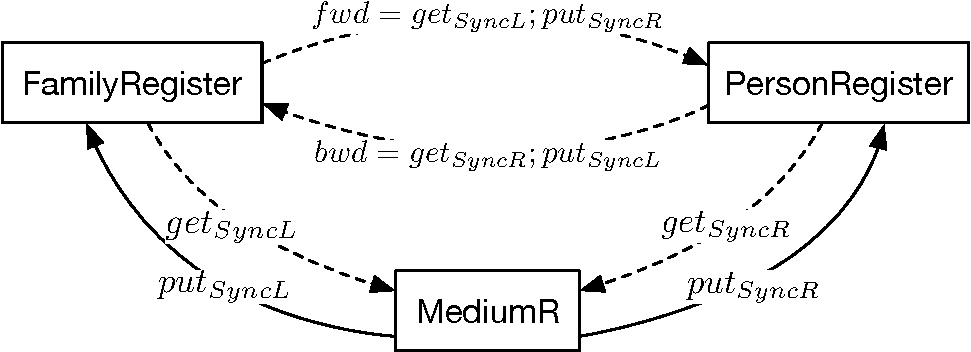
\includegraphics[width=\columnwidth]{diagrams/solutions/bigulSolnOverview}
    \caption{Handling a symmetric bx with BiGUL}
    \label{fig:bigulSolnOverview}
\end{figure}
%
In this decomposition, an additional data structure \texttt{MediumR} is introduced and can be thought of intuitively as the intersection of both data structures, i.e., it contains exactly the concepts that are present in both the source and target model spaces and that must be kept consistent.
All the bx developer now has to do is program how \texttt{MediumR} models can be \emph{put} into \texttt{Person\-Regis\-ter} models via $put_{SyncR}$, and into \texttt{Family\-Regis\-ter} models via $put_{SyncL}$.
The required \emph{fwd} and \emph{bwd} transformations can now be computed as depicted in figure~\ref{fig:bigulSolnOverview} by composing programmed \emph{put} and derived \emph{get} arrows as required.\footnote{The actual solution is a bit more complex as \emph{SyncL} is further decomposed into two arrows.}

To provide some details for actual BiGUL code, figure~\ref{fig:bigulSolnDetails} depicts the BiGUL program for $put_{SyncR}$.
Recall that the architecture for this solution is restoration-based (with $hAln$) for an initial-state-based scenario.
So this code conceptually represents \emph{fCR} and $hAln$ (see figure~\ref{fig:initialStateBased}).
The parts of the code representing $hAln$ are in black with a white background, while parts representing \emph{fCR} are in white with a black background.

\begin{figure}[tbp]
    \centering
    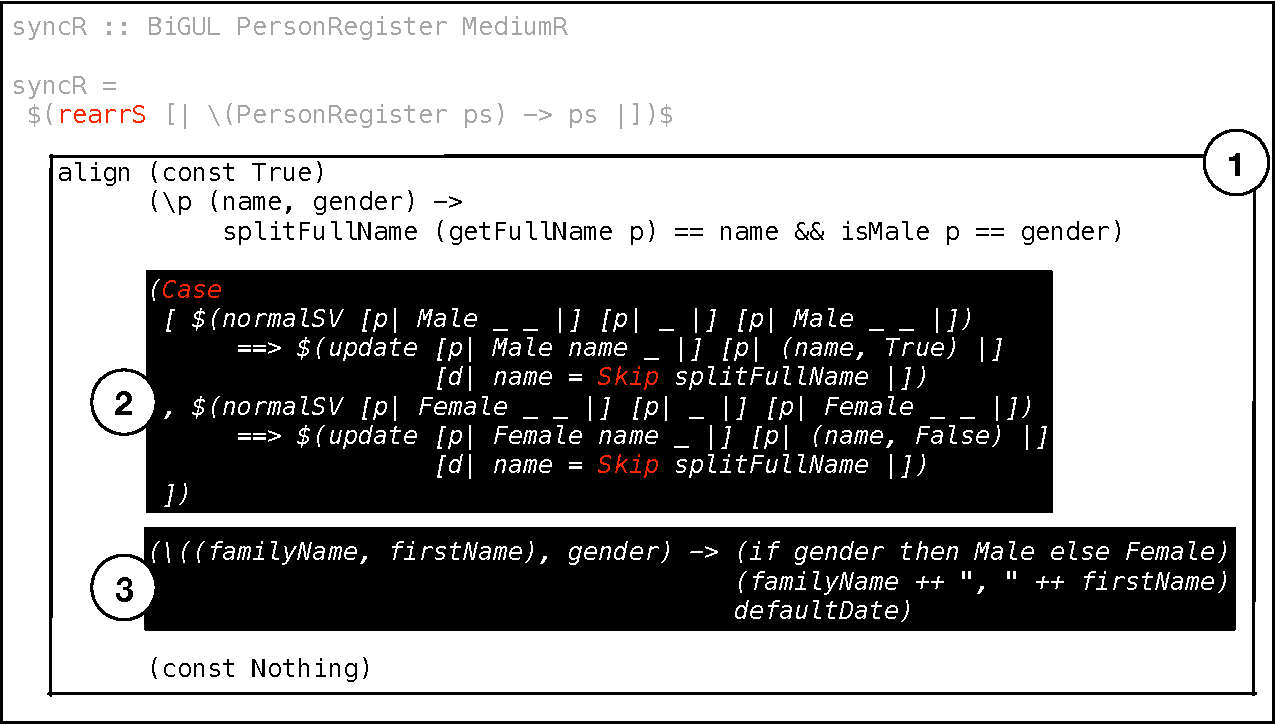
\includegraphics[width=\columnwidth]{diagrams/solutions/bigulSolnDetails}
    \caption{Structure of a BiGUL program}
    \label{fig:bigulSolnDetails}
\end{figure}

As both models are essentially lists (of persons and $(name, gender)$ pairs) $hAln$ can be implemented with the auxiliary function \texttt{align} that takes a matching condition and uses it to lift a BiGUL program on elements to lists (marked with label 1 in figure~\ref{fig:bigulSolnDetails}).
The simple strategy is to traverse the list of view elements and to search for the first source element that matches according to the condition (here simply a comparison of name and gender).
If a match is found then the first part of the \emph{fCR} code (label 2) is executed (it does nothing as the elements are already consistent), if no match can be found then a new source element is created using the second part of the \emph{fCR} code (label 3).
If unmatched source elements remain after all view elements have been matched, they are simply deleted by \texttt{align}.

Finally, although the code might appear cryptic without looking up all details, the used BiGUL primitives are highlighted red in figure~\ref{fig:bigulSolnDetails}.
The point here is that the entire program is a composition of primitives, designed in a way that this resembles programming in a standard (imperative) programming language.


\subsection{BXtend}
\label{sec:BXtend}

\NOTE{\emph{Solution expert:} Thomas, \emph{Interviewer:} Tony}

Classification according to our feature model:

style:  restoration-based
application scenario:  initial-diag-based
well-behavedness guarantees: none
consistency relation: implicit
synchronization: on-demand, explicit control

Extra details concerning architecture:

Applies restoration-based architecture depicted in figure~\ref{fig:initialDiagBased}.
\emph{fCR/bCR} is decomposed into multiple ``rules'' consisting of restoration logic separated into forward and backward direction.
Each rule defines flexibly, e.g., based on a certain type, if it is applicable or not.
Similarly, each rule checks first by exploiting the supplied corr if existing structure in the dependent model can be reused, suitably changed, or deleted and created as required.
To perform \emph{fCR/bCR} an orchestration component is supplied to decide the order in which individual rules are applied and combined to realize \emph{fCR/bCR}.
This global component can also perform a final clean up if this is required.
The delta created as output is mixed in the sense that each rule can already perform deletion and creation as required.

Technical, language-related points:

Xtend is used as implementation language to provide a compact, readable syntax.
As Xtend integrates seamlessly with Java, Java can also be used in the implementation.

Conclusion:

+ flexible, solutions can be made very efficient, full control over the synchronization process, low learning curve

- no guarantees, solutions can be just as inefficient if preconditions of rules are costly to check (as this is checked for the entire model) => a bad programmer can produce unreadable, inefficient, and incompatible \emph{fCR/bCR}.

\subsection{eMoflon}
\label{sec:eMoflon}

\NOTE{\emph{Solution expert:} Tony, \emph{Interviewer:} Zinovy}

TODO

\subsection{EVL+STrace}
\label{sec:EVLPlusSTrace}

\NOTE{\emph{Solution expert:} Leila , \emph{Interviewer:} Thomas}

\subsection{JTL}
\label{sec:JTL}

\NOTE{\emph{Solution expert:} Romina, \emph{Interviewer:} Tony}

TODO

%\clearpage

\subsection{NMF Synchronizations}
\label{sec:NMF}

\NOTE{\emph{Solution expert:} Georg, \emph{Interviewer:} Bernhard}

\subsubsection{Approach}
\label{sec:ApproachNMF}

NMF Synchronizations \cite{SoSyM2017-Hinkel}is a bx language which is formally based on category theory. Consistency between two models is defined in terms of consistency relations between their elements. In the case of mutual consistency, an element-level consistency relation is an \emph{isomorphism} between typed source and target elements, i.e., a bijective mapping between elements of some type $A$ in the source model and elements of some type $C$ in the target model satisfying specified consistency constraints. Consistency relations are coupled: For an $A$-element to be consistent with a $C$-element, an isomorphism between dependent source and target elements (of types $B$ and $D$)may be required. In addition to defining element-level consistency relations, consistency restoration has to be specified, provided that no default restoration is available.

\begin{figure}[tb!]
	\centering
	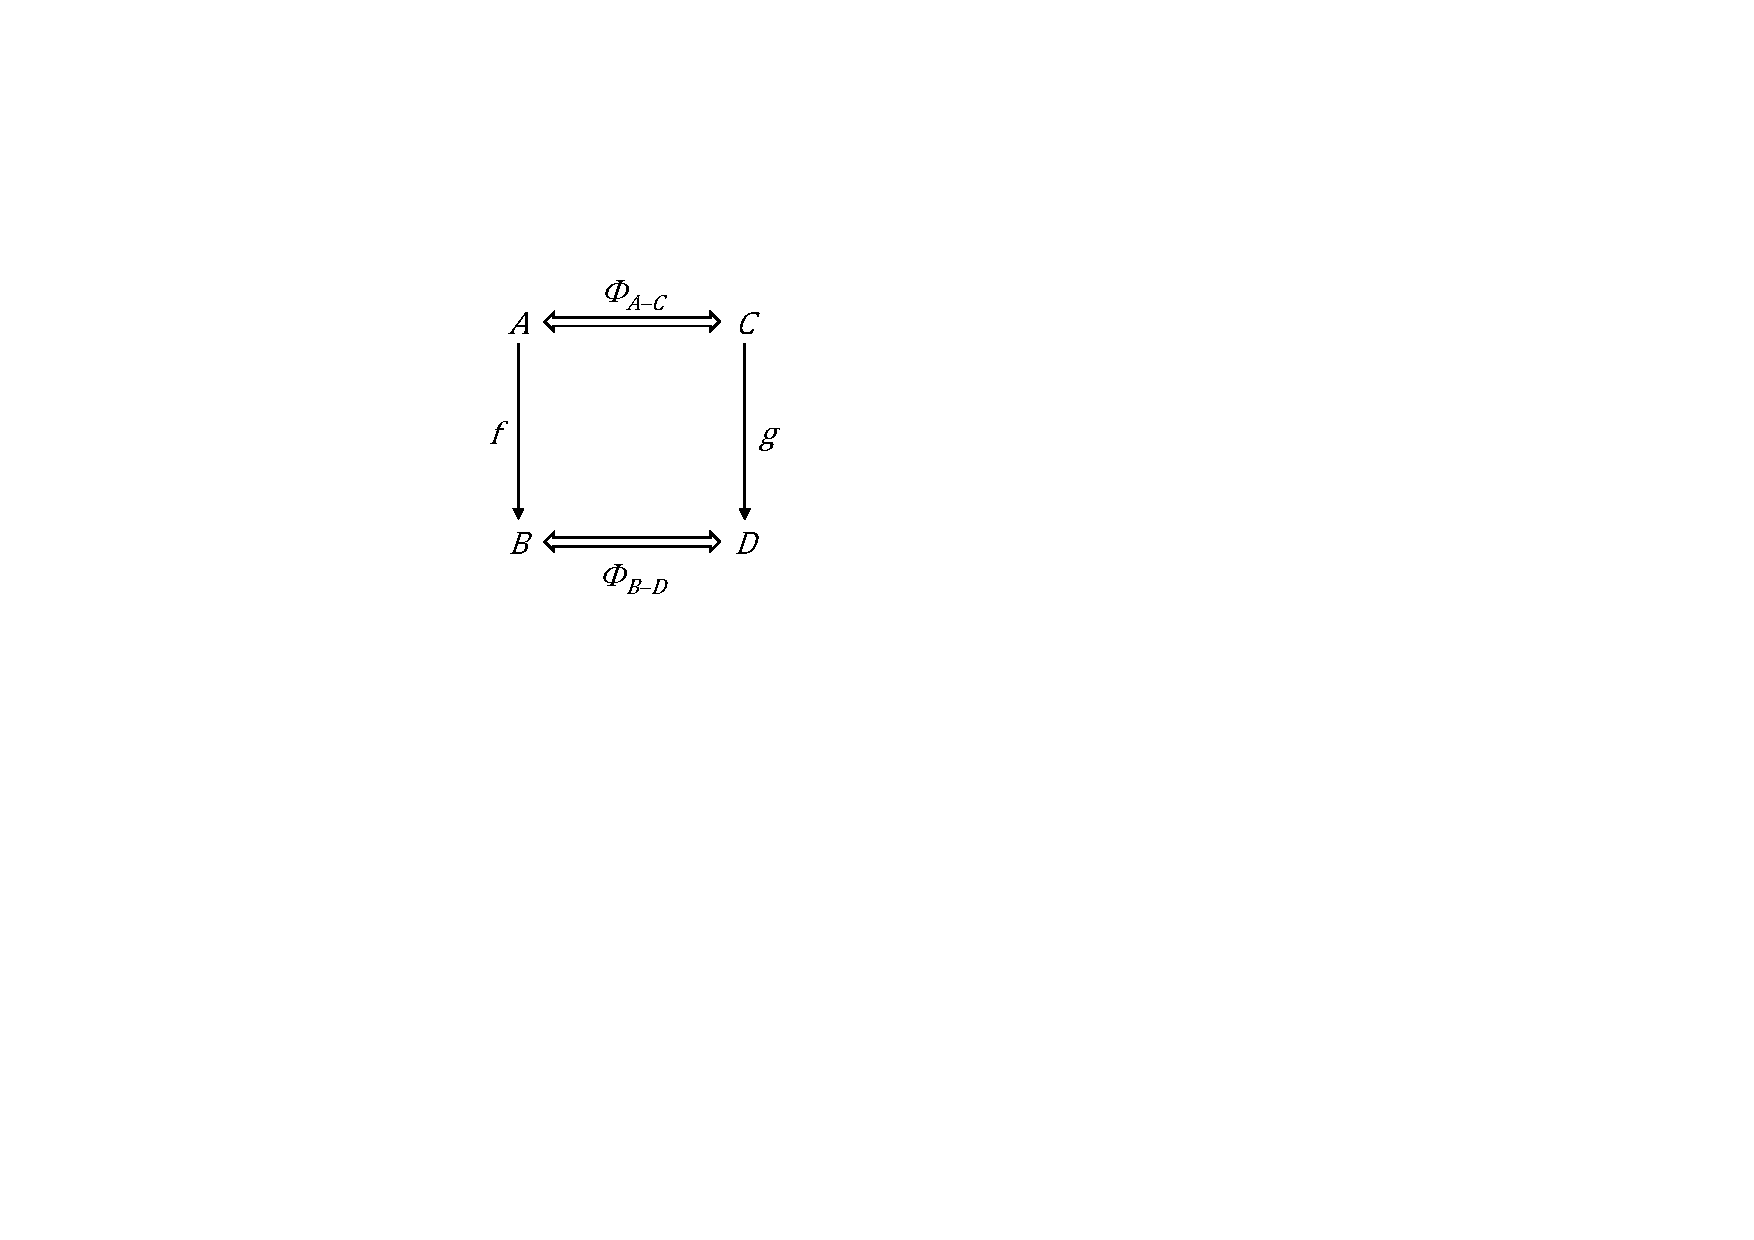
\includegraphics[width=0.35\columnwidth]{diagrams/NMFSynchronizationBlock}
	\caption{Schematic view of a synchronization block}
	\label{fig:SynchronizationBlock}
\end{figure}

The overall synchronization is specified in terms of \emph{synchronization blocks}, which are illustrated schematically in Figure~\ref{fig:SynchronizationBlock}. The isomorphisms mentioned above are represented by horizontal arrows. The isomorphism $\varPhi_{A-C}$ on the top is called \emph{base isomorphism}, while $\varPhi_{B-D}$ at the bottom plays the role of the \emph{target isomorphism}. A target isomorphism may occur as base isomorphism in another synchronization block, resulting in nested synchronization blocks. Furthermore, an isomorphism may play the role of a base isomorphism in multiple synchronization blocks, meaning that multiple consistency relations are required for making a pair of elements in the base isomorphism consistent.

The vertical arrows labeled with $f$ and $g$ denote \emph{intra-model lenses}. An intra-model lense is composed of a pair of functions called \emph{Get} and \emph{Put}. \emph{Get} and \emph{Put} are queries and updates on model elements --- in the simplest case getters and setters of element properties --- which have to satisfy round-trip laws: (1) Putting the result returned from a \emph{Get} does not change the state of the model; (2) Getting a value after a \emph{Put} returns the argument passed to the \emph{Put} operation.

Depending on the results returned from \emph{Get} operations, synchronization blocks may be classified into single-and multi-valued blocks. In the case of a \emph{single-valued block}, the \emph{Get} functions return single values which have to be consistent (e.g., the values are required to be equal). For a \emph{multi-valued block}, the \emph{Get} functions return collections. In this case, an isomorphism between these collections must be established.

The consistency relation between two models is defined by the synchronization blocks, using only the \emph{Get} operations. For consistency restoration, the \emph{Put} operations, are required, as well. For example, in a forward transformation the \emph{Get} operations on the source model are needed to retrieve the source model elements with which consistency has to be established in the target model. For updating the target model, the corresponding \emph{Put} operations are required. In simple situations, a \emph{Put} operation may be derived from the \emph{Get} operation. Otherwise, the transformation developer has to provide an explicit specification of \emph{Put} satisfying the round-trip laws of intra-model lenses. 

Altogether, the transformation developer defines the consistency relation declaratively in a functional style with the help of synchronization blocks and their \emph{Get} operations. This specification is complemented with the provision of \emph{Put} operations, which are written in a procedural style. A single specification suffices to define mutual consistency; in this regard, NMF Synchronizations is a bidirectional language. This specification is complemented with unidirectional procedural parts defining how consistency is restored in forward and backward direction, respectively.

\subsubsection{Solution}
\label{sec:solutionNMF}

NMF Synchronization is an \emph{internal DSL} based on the host language C\#. The following description is based on the solution in NMF Synchronizations submitted to TTC 2017 \cite{Hinkel2017}. Listing~\ref{lst:nmf} shows fragments of this solution, to be explained below. Since NMF Synchronization is a part of \emph{NMF} \cite{Hinkel2016}, the .NET Modeling Framework, the solution to the Families to Persons benchmark runs in a separate process which communicates with the EMF-based Benchmarx process via data streams. Below, we will not explain how this coupling is implemented; rather, we will focus on the actual core solution.



\lstdefinelanguage{cs}{
	morekeywords = {using,namespace,class,override,void,null,public,protected,private,static,out,bool,string,return,var,new,true,false,if,else,as},
	morecomment=[l]{--},
	morecomment=[s]{/*}{*/}
}


\begin{lstlisting}[label={lst:nmf}, float=*t, language=cs, caption={Solution in NMF Synchronizations}]
namespace TTC2017.FamiliesToPersons.NMF {
    public class FamiliesToPersonsSynchronization : ReflectiveSynchronization {
        public class FamilyRegisterToPersonRegister : SynchronizationRule<FamilyRegister, PersonRegister> {
            public override void DeclareSynchronization() {
                SynchronizeMany(SyncRule<MemberToMember>(),
                    fam => new FamilyMemberCollection(fam),
                    persons => persons.Persons);
            }
        }

        public class MemberToMember : SynchronizationRule<IFamilyMember, IPerson> {
            public override void DeclareSynchronization() {
                Synchronize(m => m.GetFullName(), p => p.Name);
            }
        }
        
        public class MemberToFemale : SynchronizationRule<IFamilyMember, IFemale> {
            public override void DeclareSynchronization() {
                MarkInstantiatingFor(SyncRule<MemberToMember>(), 
                    leftPredicate: m => m.MotherInverse != null || m.DaughtersInverse != null);
            }
            ...
        }
        
        private class FamilyMemberCollection : CustomCollection<IFamilyMember> {
            ...
            public override void Add(IFamilyMember item) {
                var temp = item.GetExtension<TemporaryStereotype>();
                item.AddToFamily(Register, temp.IsMale, temp.LastName);
                item.Extensions.Remove(temp);
            }
            ...
        }
        ...
    }
}
\end{lstlisting} 

In NMF Synchronizations, a transformation is defined by extending classes from a library. In Listing~\ref{lst:nmf}, the overall transformation is defined by a single top-level class (starting at line~2) containing further nested classes.

A \emph{synchronization rule} includes all synchronization blocks sharing the same base isomorphism. In the Families to Persons benchmark, each synchronization rule contains just one synchronization block. A synchronization rule is defined by subclassing the generic class \code{SynchronizationRule} (lines~3, 11, and 17). This class is equipped with two generic parameters for the types of the source and the target elements of the base isomorphism, respectively. The actual synchronization blocks are defined by overriding the method \code{Declare\-Synchron\-ization} (lines~4, 12, and 18). 

Altogether, the class starting at line~3 defines a multi-valued synchronization block with a base isomorphism between the roots of the families model and the persons model (of type \code{FamilyRegister} and \code{Person\-Register}, respectively) and a target isomorphism between family members and persons. The call to the method \code{SynchronizeMany} specifies the nested synchronization rule \code{MemberToMember}, as well as the \emph{Get} functions for retrieving the collections of family members and persons as Lambda expressions. 

\code{persons.Persons} is an \emph{invertible expression}: Since the \emph{Get} function merely collects the elements obtained via a multi-valued reference, the updates may be inferred automatically. In contrast, a \emph{custom collection} is required at the opposite end, which is implemented in the helper class \code{FamilyMemberCollection} (line~25). The implementation of the helper class has to define the path for getting the elements of the collection (traversing references to families and members sequentially), which is not shown here, and has to provide an update method for adding a family member to the collection (line~27). This \code{Add} method is required in a backward transformation to insert an already created family member at the appropriate location into the families model. To this end, a custom method \code{AddToFamily} is called (line~29) which performs this insertion depending on the configuration parameters \code{PreferExistingToNew\-Family} and \code{PreferParentToChild}. The information on the gender and the last name of the family member is retrieved from temporary stereotypes attached to the model element (line~28); these stereotypes are removed in line~30.

\code{MemberToMember} defines a single-valued synchronization block which demands that the full name of the family member be synchronized with the name of the person (i.e., the respective strings must be equal). The method \code{GetFullName} composes the full name from the first name and the last name in a straightforward way. In addition to this \emph{Get} function, we need to supply the corresponding \emph{Put} to complete the definition of the intra-model lense. To this end, a custom method \code{SetFullName} is defined which sets the full name, potentially moving the member to a different family (both methods are not shown due to the lack of space).

Finally, we need to take care of the fact that the class \code{Person} is abstract and thus cannot be instantiated in forward direction. This is achieved by two synchronization rules, one of which is shown in line~17. The rule \code{MemberToFemale} refines the rule \code{MemberToMember} by defining the type to be instantiated. Please note that the base isomorphism of the synchronization is refined to \code{IFemale} on the persons model. Furthermore, the method call in line~19 defines the predicate which has to be satisfied in order to apply this refinement (the member must be a mother or a daughter).  




\begin{figure*}[htb!]
	\centering
	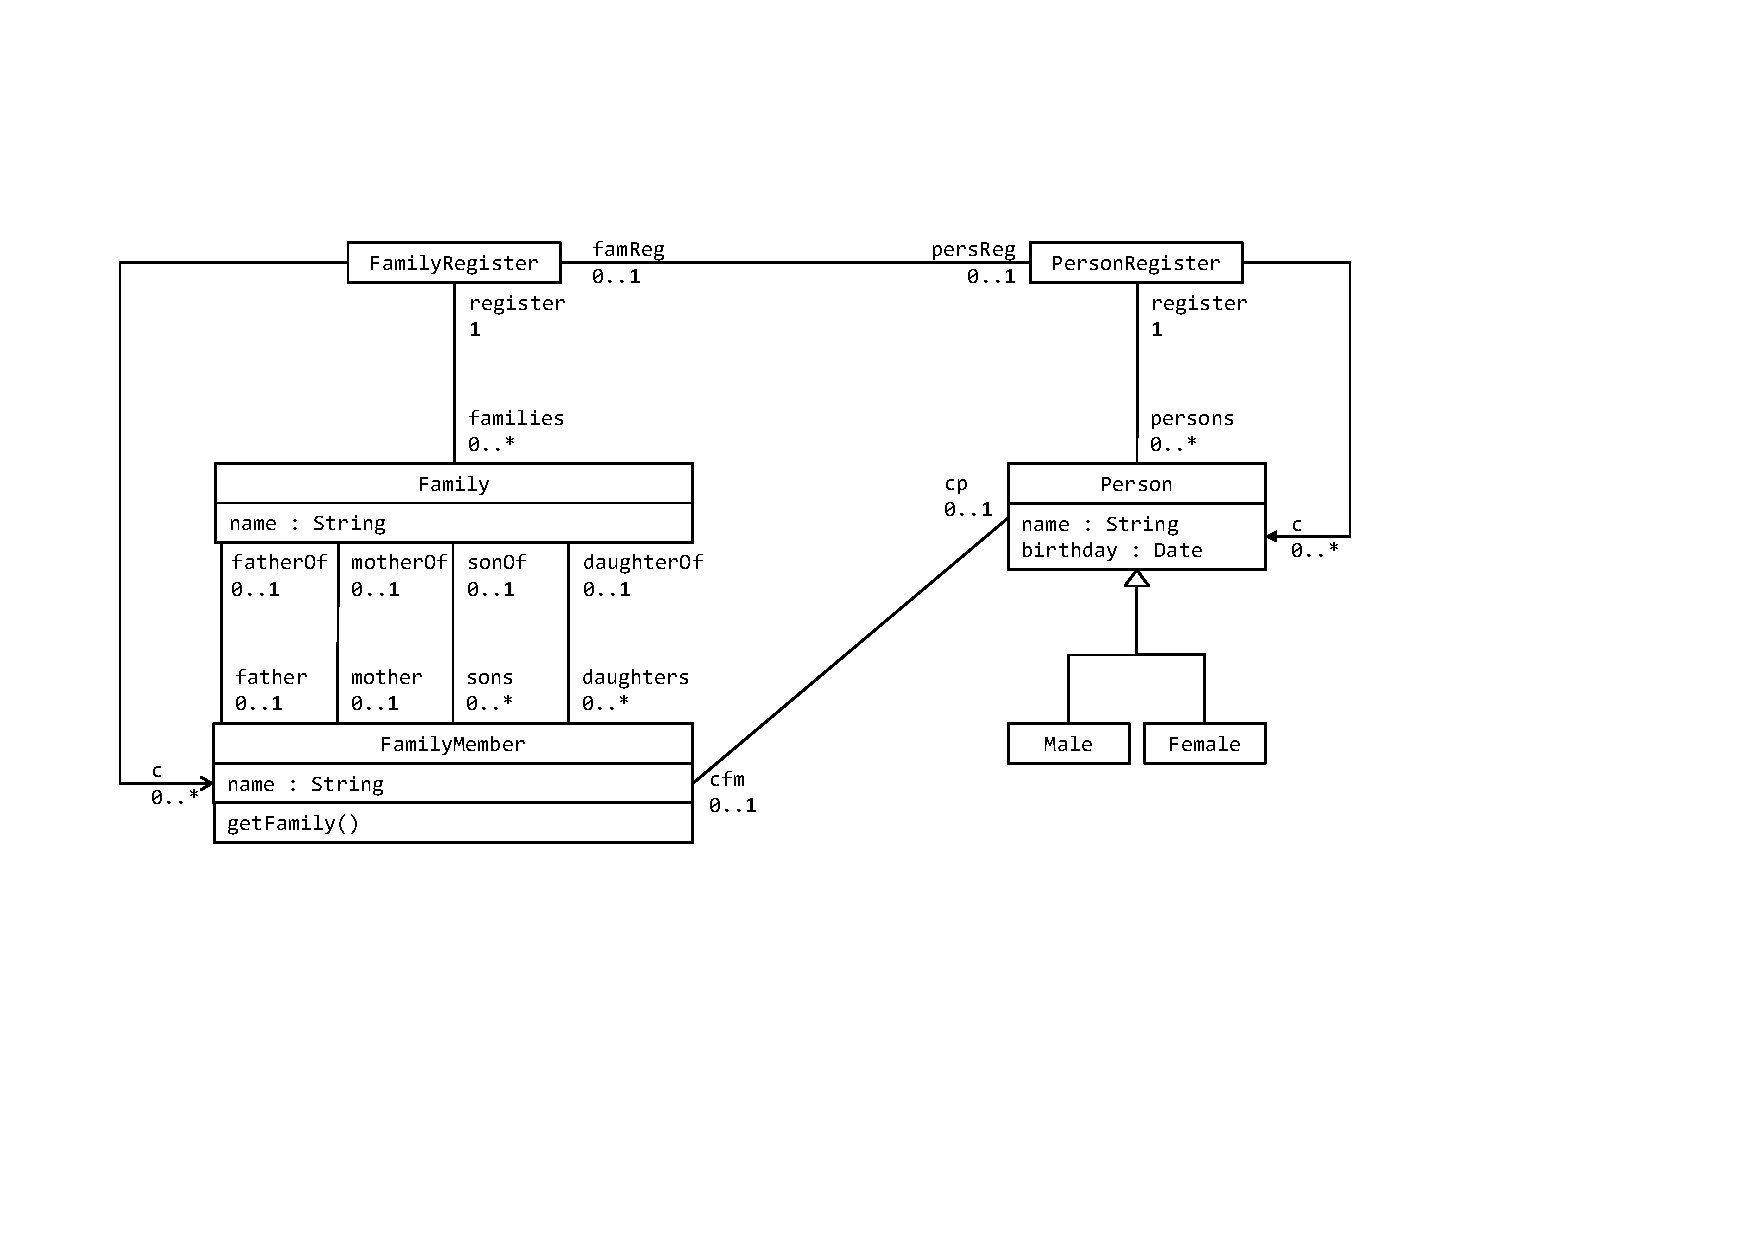
\includegraphics[width=0.75\textwidth]{diagrams/solutions/SDMLibModel}
	\caption{SDMLib model used for the benchmark}
	\label{fig:SDMLibModel}
\end{figure*}

\subsection{SDMLib}
\label{sec:SDMLib}

SDMLib, short for \emph{Story Driven Modeling Library}\footnote{http://www.sdmlib.org}, is a Java library to support Story Driven Modeling~\cite{Norbisrath2013}, a formalism based on graph transformations~\cite{Ehrig2006}.
SDMLib provides an internal DSL with Java as a host language.
Although SDMLib is not a bx tool, in the sense that it does not provide any extra support especially for developing bx, it is nonetheless included here as a ``general purpose'' model transformation tool against which bx tools should also be compared. 

As models can be viewed as attributed, typed \emph{graphs}, model transformations can also be regarded as a problem in the domain of graph transformations.
A \emph{graph rewrite rule} specifies the replacement of a graph pattern (left-hand side) by a subgraph to be embedded into the overall host graph.
Graph rewrite rules can be used to specify not only in-place model transformations, but also 
model-to-model transformations by applying the rules to multiple graphs.
Graph rewrite rules are \emph{declarative} in the sense that the exact order in which to traverse the host graph and check for or replace patterns is not specified.


\subsubsection{Classification}
The solution to the benchmark with SDMLib follows a \emph{restoration-based} architectural style; \emph{fCR} and \emph{bCR} are implemented with graph rewrite rules. 

The solution addresses the \emph{initial-diag-based} application scenario (figure \ref{fig:initialDiagBased}).
A diag is taken as input, and the dependent model is manipulated until both models are consistent again. 

No formal guarantees are provided by SDMLib as \emph{fCR} and \emph{bCR} are specified separately and independently.
It is left up to the transformation developer to ensure that the implementations are not contradictory.
As with the BXtend solution, this can be viewed as an advantage; the bx programmer may freely decide whatever is necessary to solve the current task.

The SDMLib solution has no explicit notion of \emph{consistency} as it is \emph{implicitly} given by the implemented pair of \emph{fCR/bCR}.
Accordingly, synchronization \emph{control} is \emph{explicit}, and programmed by providing suitable graph rewrite rules.
The SDMLib solution was developed with the benchmark in mind and thus supports \emph{directed}, \emph{on demand}, \emph{automatic} synchronization. 

\subsubsection{Benchmark solution with SDMLib}

The following description is based on the SDMLib solution for the Families-to-Persons benchmark at TTC 2017~\cite{Zundorf2017}.
As SDMLib is designed for in-place transformations on a single host graph, the solution uses a single metamodel as depicted in figure~\ref{fig:SDMLibModel}.
To support incrementality efficiently, additional unidirectional references between \code{FamilyRegister} and \code{Fami\-lyMember}, and \code{PersonRegister} and \code{Person} are used to detect changed elements.
Finally, the correspondences are represented using two bidirectional references.
The SDMLib solution thus operates on a single graph comprising the contents of both models as well as explicit correspondence links between respective elements. 

\begin{lstlisting}[label={lst:sdmlib}, float=hbt!, language=java, caption={Forward transformation in SDMLib}]
private void transformForward() {
 familyRegisterPO = new FamilyRegisterPO()
   .withPatternObjectName("fr");
 PersonRegisterPO personRegisterPO = 
  familyRegisterPO.createPersonRegisterPO()
                  .withPatternObjectName("pr");
 FamilyMemberPO memberPO = familyRegisterPO
   .createCPO()
   .withPatternObjectName("fm");

 // there is an old corresponding person
 memberPO.startSubPattern();
 PersonPO oldPersonPO = memberPO.createCpPO()
   .withName("oldP");
 oldPersonPO.createCondition(p -> 
   ensureNameAndGender(p));
 memberPO.endSubPattern();

 // no corresponding person
 memberPO.startNAC();
 memberPO.createCpPO()
   .withPatternObjectName("noOldP");
 memberPO.endNAC();
 MalePO personPO = memberPO
   .createCpMalePO(Pattern.CREATE)
   .withPatternObjectName("newP");
 personPO.createRegisterLink(
   personRegisterPO, 
   Pattern.CREATE);
 personPO.createCondition(p -> 
   ensureNameAndGender(p));
    
 familyRegisterPO.createLink(
   memberPO, 
   Pattern.DESTROY);

 familyRegisterPO.rebind(familyRegister);
 familyRegisterPO.doAllMatches();	    
}
\end{lstlisting}

The core of the SDMLib solution consists of two graph rewrite rules, one for each direction.
While graph rewrite rules are typically presented using a visual concrete syntax, we use the actual textual concrete syntax provided by the tool to enable and simplify a comparison with all other solutions.  

Listing~\ref{lst:sdmlib} depicts the graph rewrite rule for the forward transformation using SDMLib's internal DSL, embedded into Java.
The method for the graph rewrite rule uses code generated from the graph metamodel depicted in figure~\ref{fig:SDMLibModel}. 

The statements on line~2--9 define story pattern objects for the family register, the person register, and a family member, which need to be matched in the families model; the links connecting these objects are added implicitly to the story pattern by the invoked methods (e.g., \code{createCPO()}). 

Lines~12-17 handle the case that a corresponding person object already exists.
This case is realized with an optional subpattern, which is started at line~12 and is terminated at line~17.
The pattern is composed of an old person object, connected to the family member object by a correspondence link.
If pattern matching succeeds, the method \code{ensure\-Name\-And\-Gender} is invoked to restore consistency.

Lines~20--31 deal with the case where there is no corresponding person object.
This is handled with a \emph{negative application condition}, defined on lines~20--23.
On lines~17--19, elements of story patterns are created that define the actions to be performed when the negative application condition holds: A person object has to be created and linked to the person register; the method \code{ensure\-Name\-And\-Gender} is then called to establish consistency with the family object.

Finally, the temporary link between the family register and the family member --- which is set in the course of changes to the families model --- is matched and then removed (lines~33--35), the story pattern object for the family register is bound (line~37), and the pattern is applied to all matches (line~38).

%%% Local Variables:
%%% mode: latex
%%% TeX-master: "../main"
%%% End:


%%% Local Variables:
%%% mode: latex
%%% TeX-master: "../main"
%%% End:
